\section{Evaluation}
\label{sec:eval}

We have implemented our approach in \toolname: a system for
repairing parse errors for \python at its entirety. Next,
we describe our implementation and an evaluation that addresses three
questions:

\begin{itemize}
    \item \textbf{RQ1}: How \emph{accurate} are \toolname's predicted error production rules?
                        (\S~\ref{sec:eval:accuracy})
    \item \textbf{RQ2}: How \emph{precisely} can \toolname repair parse errors?
                        (\S~\ref{sec:eval:precise})
    \item \textbf{RQ3}: How \emph{efficiently} can \toolname repair parse errors?
                        (\S~\ref{sec:eval:efficiency})
    \item \textbf{RQ4}: How \emph{useful} are \toolname's suggested repairs?
                        (\S~\ref{sec:eval:useful})
    % \item \textbf{RQ4}: How \emph{precise} are \toolname's template fixes?
    %                     (\S~\ref{sec:eval:template_quality})

\end{itemize}

% \subsection{Implementation} \label{sec:eval:gen_method}

\mypara{Training Dataset}
%
For our evaluation, we use a \python dataset gathered from
PythonTutor.com~\citep{Guo2013} between 2017 and 2018, previously used in
related work \citep{Endres2019,Cosman2020}. Each program which throws an
uncaught Python exception is paired with the next program by the same user that
does not crash, under the assumption that the latter is the fixed version of the
former. We discard pairs where the difference between crashing and fixed
versions is too high (more than a standard deviation above average), since these
are usually unrelated submissions or complete refactorings. We also discard
submissions that violate PythonTutor's policies (e.g., those using forbidden
libraries). Ultimately, the dataset used in this evaluation contains almost a
million usable program pairs, representing students from dozens of universities
(PythonTutor has been used in many introductory courses~\citep{Guo2013}) as well
as non-traditional novices.

\mypara{Dataset labeling}
%
\toolname represents each program with its abstracted token sequence $t^a$ for
the training procedure. For the full set of \python there are \emph{360 terminal
error production rules} that \toolname's has to predict from.

% \mypara{Dataset Cleaning}
% %
% We extract fixes as expressions replacements over a program pair using
% $\diffsym$ A disadvantage of using $\diffsym$s with this dataset is that some
% students may have made many, potentially unrelated, changes between
% compilations; at some point the ``fix'' becomes a ``rewrite''. These rewrites
% can lead to meaningless fix templates and error locations. We discard such
% outliers when the fraction of subexpressions that have changed in a program is
% more than one standard deviation above the mean, establishing a
% $\diffsym$ threshold of 40\%. We also discard programs that have changes in 5 or
% more locations, noting that even state-of-the-art multi-location repair
% techniques cannot reproduce such ``fixes'' \citep{Saha_2019}. The discarded
% changes account for roughly 32\% of each dataset, leaving 2,475 program pairs
% for \SPRING and 2,177 pairs for \FALL. Throughout, we use \SPRING as a training
% set and \FALL as a test set.

% \mypara{\dnn based Classifier}
% %
% \toolname's template prediction uses a multi-layer neural network \dnn based
% classifier with three fully-connected hidden layers of 512 neurons. The neurons
% use rectified linear units (ReLU) as their activation function
% \citep{Nair2010-xg}.
% %
% The \dnn was trained using \emph{early stopping} \citep{Hastie2009-bn}: training
% is stopped when the accuracy on a distinct small part of the training set is not
% improved after a certain amount of epochs (5 epochs, in our implementation).
% %
% We set the maximum number of epochs to 200.
% %
% We used the \textsc{Adam} optimizer \citep{Kingma2014-ng},
% a variant of stochastic gradient descent that converges faster.

\subsection{RQ1: Accuracy}
\label{sec:eval:accuracy}

We consider \toolname's transformer classifiers' accuracy up to the \emph{top
50} error production rules predictions against our original and the final
version of our approach

% colors from http://colorbrewer2.org/?type=sequential&scheme=Blues&n=3
\definecolor{blue1}{HTML}{DEEBF7}
\definecolor{blue2}{HTML}{9ECAE1}
\definecolor{blue3}{HTML}{3182BD}
\definecolor{green1}{HTML}{E5F5E0}
\definecolor{green2}{HTML}{A1D99B}
\definecolor{green3}{HTML}{31A354}

\begin{figure}[t]
  % \begin{minipage}[c]{0.49\linewidth}
    \centering
    \resizebox{0.6\linewidth}{!}{
      \Large
      \begin{tikzpicture}
      \begin{axis}[
        ybar stacked,
        width=1.1\linewidth,
        height=11cm,
        % title={Accuracy of Repair Template Prediction},
        ylabel={Prediction Accuracy (\%)},
        bar width=1cm,
        ymin=0.0,
        ymax=101.0,
        ytick={0.0, 10.0, 20.0, 30.0, 40.0, 50.0, 60.0, 70.0, 80.0, 90.0, 100.0},
        yticklabel={\pgfmathparse{\tick}\pgfmathprintnumber{\pgfmathresult}},
        ytick style={draw=none},
        ymajorgrids = true,
        symbolic x coords={original, abstracted, abstracted-best},
        enlarge x limits=0.3,
        xtick=data,
        xtick style={draw=none},
        xticklabels={\textsc{Original}\xspace, \textsc{Abstracted}\xspace, \textsc{Threshold}\xspace},
        %x tick label style={rotate=45, anchor=north east},
        % x tick label style={font=\small},
        % y tick label style={font=\small},
        reverse legend,
        % transpose legend,
        legend style={legend pos = north east, legend columns=4, font=\small},
      ]

      \addplot[draw=black, fill=blue2, bar shift=-.501cm, postaction= { pattern=dots }] coordinates {(original, 0.0) (abstracted, 0.0) (abstracted-best, 79.28025102961365)};

      \resetstackedplots

      \addplot[draw=black, fill=green2, bar shift=.501cm, postaction= { pattern=dots }] coordinates {(original, 0.0) (abstracted, 0.0) (abstracted-best, 69.82968369829683)};

      \resetstackedplots

      \addplot[draw=black, fill=green1, bar shift=.501cm] coordinates {(original, 12.875536480686696) (abstracted, 58.394160583941606) (abstracted-best, 0.0)};
      \addlegendentry{Top-10}
      \addplot[draw=black, fill=green2, bar shift=.501cm] coordinates {(original, 20.100143061516448) (abstracted, 14.922952149229523) (abstracted-best, 0.0)};
      \addlegendentry{Top-20}
      \addplot[draw=black, fill=green3, bar shift=.501cm] coordinates {(original, 31.974248927038623) (abstracted, 15.49067315490673) (abstracted-best, 0.0)};
      \addlegendentry{Top-50}
      \addlegendimage{empty legend}
      \addlegendentry{Rare:}

      \resetstackedplots

      \addplot[draw=black, fill=blue1, bar shift=-.501cm] coordinates {(original, 56.712132089016514) (abstracted, 72.11217885859972) (abstracted-best, 0.0)};
      \addlegendentry{Top-10}
      \addplot[draw=black, fill=blue2, bar shift=-.501cm] coordinates {(original, 11.769733018835673) (abstracted, 9.335163757599531) (abstracted-best, 0.0)};
      \addlegendentry{Top-20}
      \addplot[draw=black, fill=blue3, bar shift=-.501cm] coordinates {(original, 18.65107852186101) (abstracted, 11.253840622344256) (abstracted-best, 0.0)};
      \addlegendentry{Top-50}
      \addlegendimage{empty legend}
      \addlegendentry{All:}

      \end{axis}
      \end{tikzpicture}
    }
    \caption{
      Results of our error production rule prediction classifiers for the simple original token sequences and their abstracted versions using the PCFG.
    }
    \label{fig:accuracy-results}
  % \end{minipage}
  % \begin{minipage}[c]{0.49\linewidth}
  %   \centering
  %   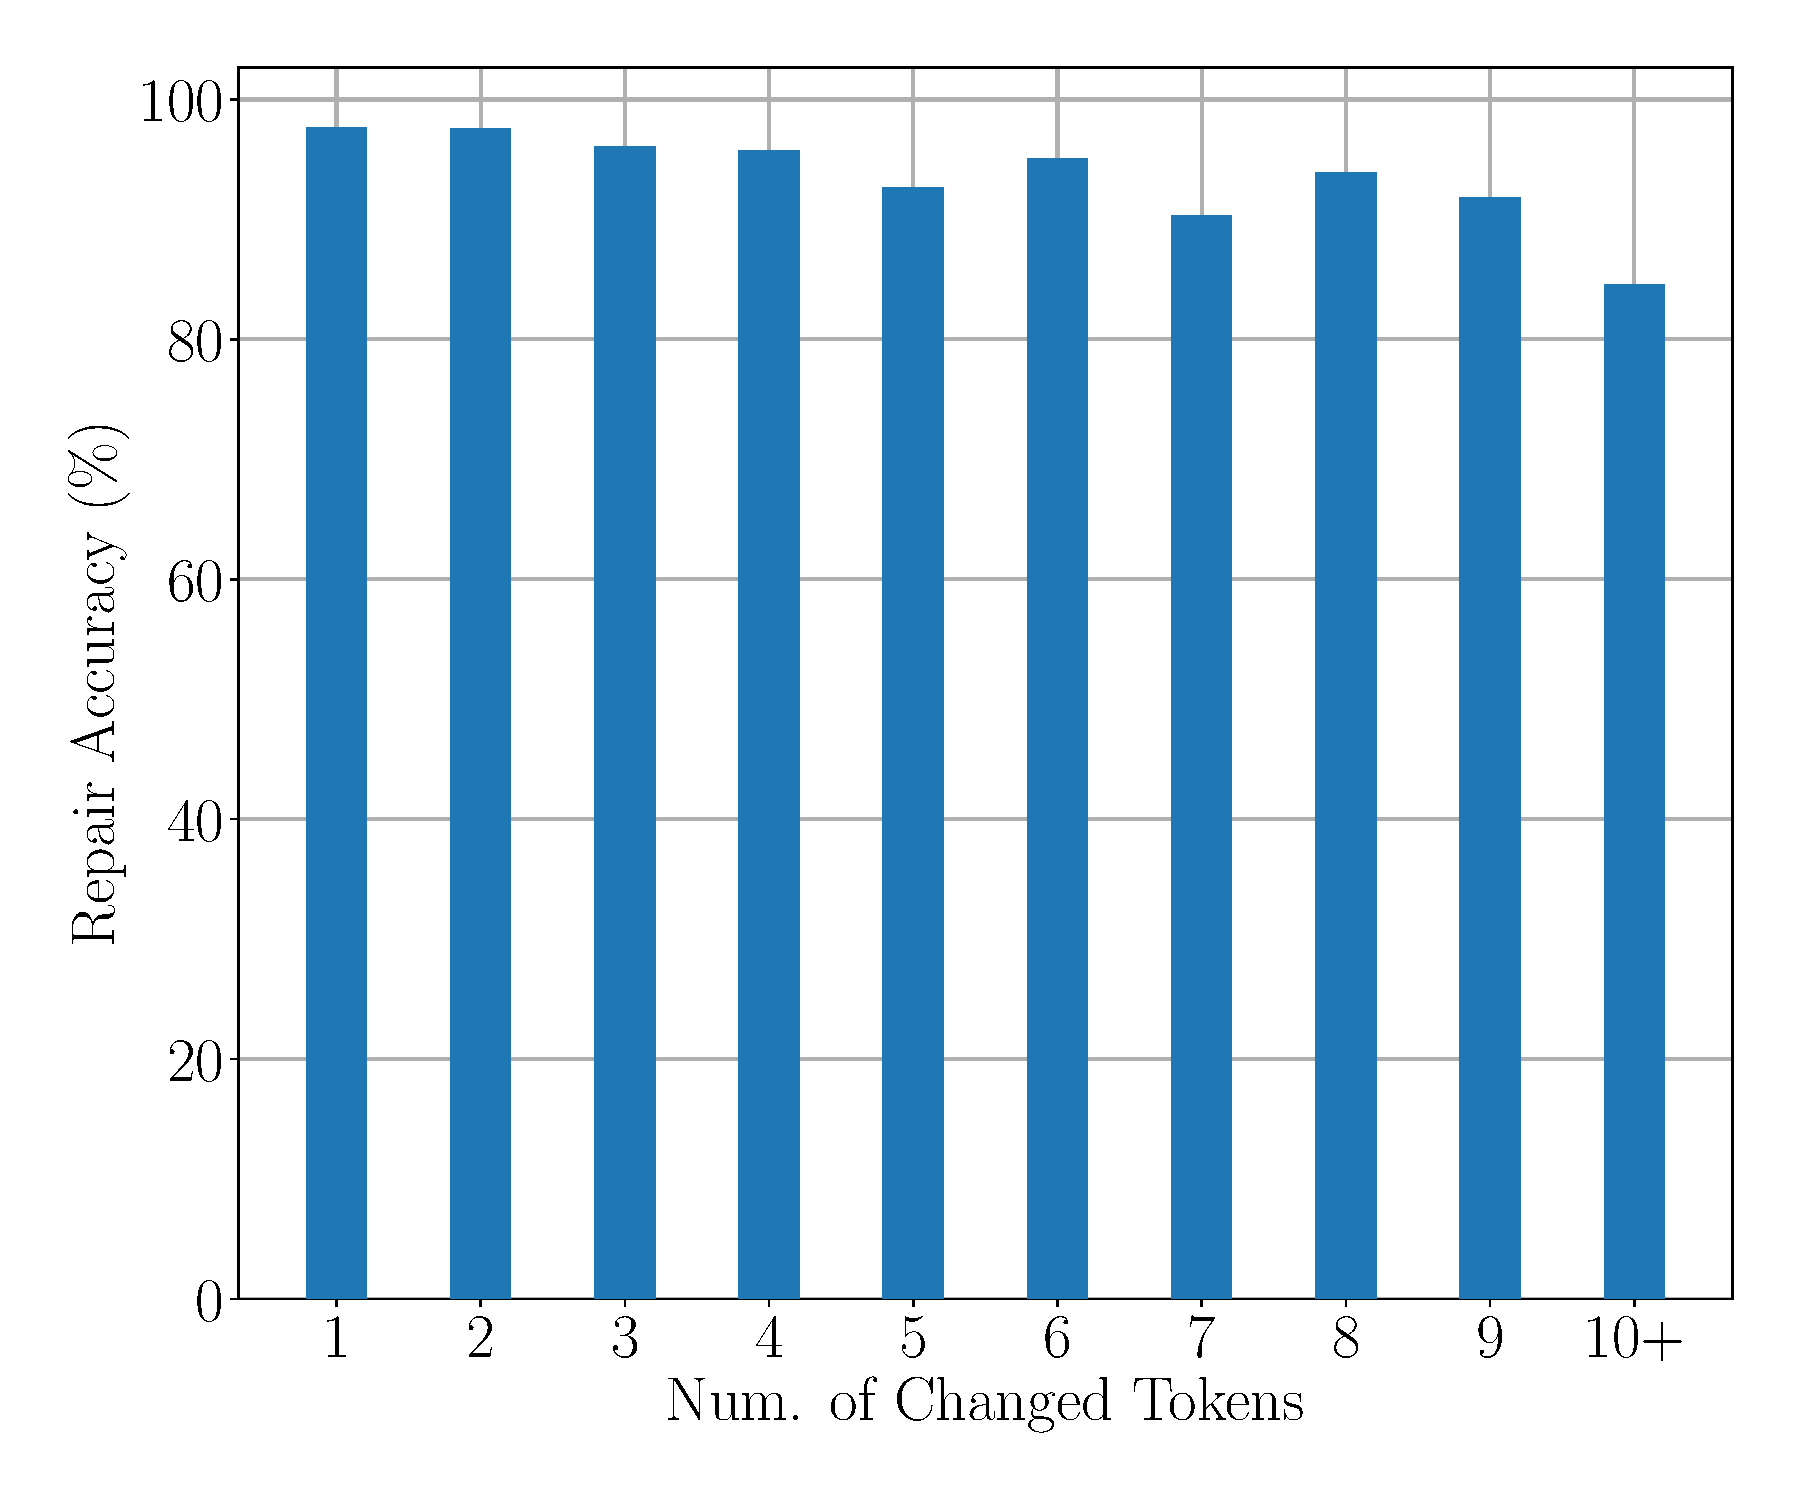
\includegraphics[width=\linewidth]{accuracy-per-change.pdf}
  %   \caption{The repair accuracy for the number of edits needed by the user to repair.}
  %   \label{fig:accuracies-per-changes}
  % \end{minipage}
\end{figure}


\mypara{Results: Accuracy of Error Rule Prediction}
%
\autoref{fig:accuracy-results} shows the accuracy results of our error
production rule prediction experiments. The y-axis describes the fraction of
programs for which the \emph{whole} set of the needed error rules needed to
repair the \emph{erroneous} program was a complete subset of the top-K predicted
rules.
%
The \textsc{Original} version of our transformer classifier didn't consider the
partial parses produced with the PCFG's aid and used the full \textsc{Original}
token sequences, whose results are presented in the first two bars of
\autoref{fig:accuracy-results}. The next two bars show our final results using
the \textsc{Abstracted} token sequences to train the classifier. Finally, the
last two dotted bars show the results for when a \textsc{Threshold} is set in
order to select the predicted error rules, instead of picking the static top-K
ones. The predicted error rule set can have a size anywhere between 1 and a
maximum of 25 (pre-defined by us based on the top-K results).

The blue bars show the accuracy on the full test set of \textsc{All} 15,000
programs, while the green bars show the results on the subset of \textsc{Rare}
programs, \ie the programs that didn't include any of the 50 most popular error
rules, that amount only for 4.8\% of our test set.

The \textsc{Original} predictor, even with the Top-50 predicted error rules is
less accurate than the Top-20 predictions of the \textsc{Abstracted}, with an
accuracy of 73.96\%, which drops to 51.16\% and 32.34\% respectively for the
Top-20 and Top-10 predictions. The \textsc{Abstracted} predictor significantly
outperforms the \textsc{Original} predictor with a 72.08\% Top-10 accuracy,
81.08\% Top-20 accuracy and 92.13\% Top-10 accuracy.

The \textsc{Threshold} predictions are almost as accurate as the
\textsc{Abstracted} Top-20 predictions with an accuracy of 79.46\% and a median
number of selected error rules of 12 (average 13.9). This could potentially mean
that this predictor is a valid alternative for the static Top-20 predictions.

Finally, we observe that our \textsc{Abstracted} classifiers generalize
efficiently for our dataset of erroneous Python programs and is almost as
accurate as the rest of the dataset with a 74.11\% Top-20 accuracy (85.69\%
Top-50 accuracy). The same holds for the \textsc{Threshold} predictions with a
72.46\% accuracy.

\begin{framed}
  \noindent \toolname's transformer classifier learns to encode programs with
  syntax errors and select candidate error production rules for them
  effectively, yielding \emph{high accuracies}. By abstracting the tokens
  sequences, \toolname is able to \emph{generalize} better and make more
  accurate predictions with a \emph{81.08\% Top-20 accuracy}.
\end{framed}


\subsection{RQ2: Repaired Program Preciseness}
\label{sec:eval:precise}

\begin{table}[t]
  \centering
  \begin{tabular}{l||cccc}
    Rules Approach                 & Parse Accuracy & User Parse Rate & Parse time & Speedup \\
    \hline
    20 Most Popular                & 79.81\% & 16.31\% & 4.8 sec  & 45.8 sec \\
    50 Most Popular                & 90.03\% & 18.55\% & 10.6 sec & 37.1 sec \\
    Top-20 (\textsc{All-Parses})   & 59.31\% & 30.57\% & 15.6 sec & 57.4 sec \\
    Top-20 (\textsc{Minimum-Cost}) & 92.45\% & 19.95\% & 4.1 sec  & 68.0 sec \\
  \end{tabular}
  \caption{Experimental results of \toolname's repair approaches.}
  \label{tab:seq2parse_full_results}
\end{table}

Next we evaluate \toolname's end-to-end accuracy and preciseness in generating
valid parses for programs with syntax errors. For all of our tests we limit the
\toolname's parsing to \emph{5 mins} and run our experiments on \emph{15,000
erroneous programs} from our dataset. The rest of the dataset was used to train
our transformer classifiers, and specifically here the \textsc{Abstracted}
classifier.

We compare our \emph{two versions} of our implementation of \toolname
(\textsc{All-Parses} and \textsc{Minimum-Cost}) against two versions of the
error-correcting parser with a static selection of the 20 and 50 most popular
error production rules in our training set. We make this comparison because we
observe in our training set that the 50 most of popular error rules are used for
parsing as much as \emph{86\%} of the dataset.

Our \textsc{All-Parses} ECEP and \textsc{Minimum-Cost} ECEP both use the
\emph{Top-20 predictions} from our \textsc{Abstracted} classifier to generate
parses and thus generate full program repairs. The \textsc{All-Parses} ECEP
keeps internally all possible states that arise from using the predicted error
rules and having a maximum repair cost of 2 edits (\ie a maximum of 2
insertions, deletions or replacements). The \textsc{Minimum-Cost} version
however keeps always the minimum-edit repair and discards all other states that
may lead to a higher cost. This allows for a higher maximum cost of 10 edits.
Finally, while \textsc{All-Parses} can generate a large number of repairs, we
keep only the top 3 repairs after filtering with a static code checker
(\textsc{Pylint} \citep{pylint2022}) as most developers will consider at most five
suggestions before falling back to manual debugging \citep{Kochhar2016-oc,
Parnin2011-ce}.

\autoref{tab:seq2parse_full_results} shows the percentage of test programs that
each of these four versions can parse successfully (\ie the parse accuracy) and
the amount of parses that match the one that user compiled. We observe that the
Top-20 predictions with the \textsc{Minimum-Cost} ECEP \emph{outperforms} every
other option in parse accuracy and parse time, with 92.45\% and 4.1 seconds
respectively. It also achieves to generate the intended parse for 19.95\% of the
set, \ie in almost 1 out 5 of the cases. The 20 most popular ECEP with 79.81\%
parse accuracy and 4.8 seconds parse time is less accurate while a bit slower in
general, and achieves 3.64\% less times to generate the user parse, while the 50
most popular is slightly less accurate with 90.03\%, but a lot slower in general
with 10.6 seconds parse time. The 50 most popular ECEP also almost achieves the
\textsc{Minimum-Cost} ECEPs with a 18.55\% user parse rate. The
\textsc{All-Parses} ECEP has a smaller parse accuracy of 59.31\%, however it
manages to generate the user fix 30.57\% of the times, \ie almost one out of
three programs with syntax errors, with the cost that is also the slowest
version with a parse time of 15.6 seconds.

\begin{framed}
  \noindent \toolname can \emph{generate parses} for \emph{92\%} of our tests
  within 4.1 secs for the majority of them, while also generating \emph{the user
  fix in almost 1 out 5 of the cases}.
\end{framed}

\subsection{RQ3: Efficiency}
\label{sec:eval:efficiency}

\begin{figure}[t]
  \centering
  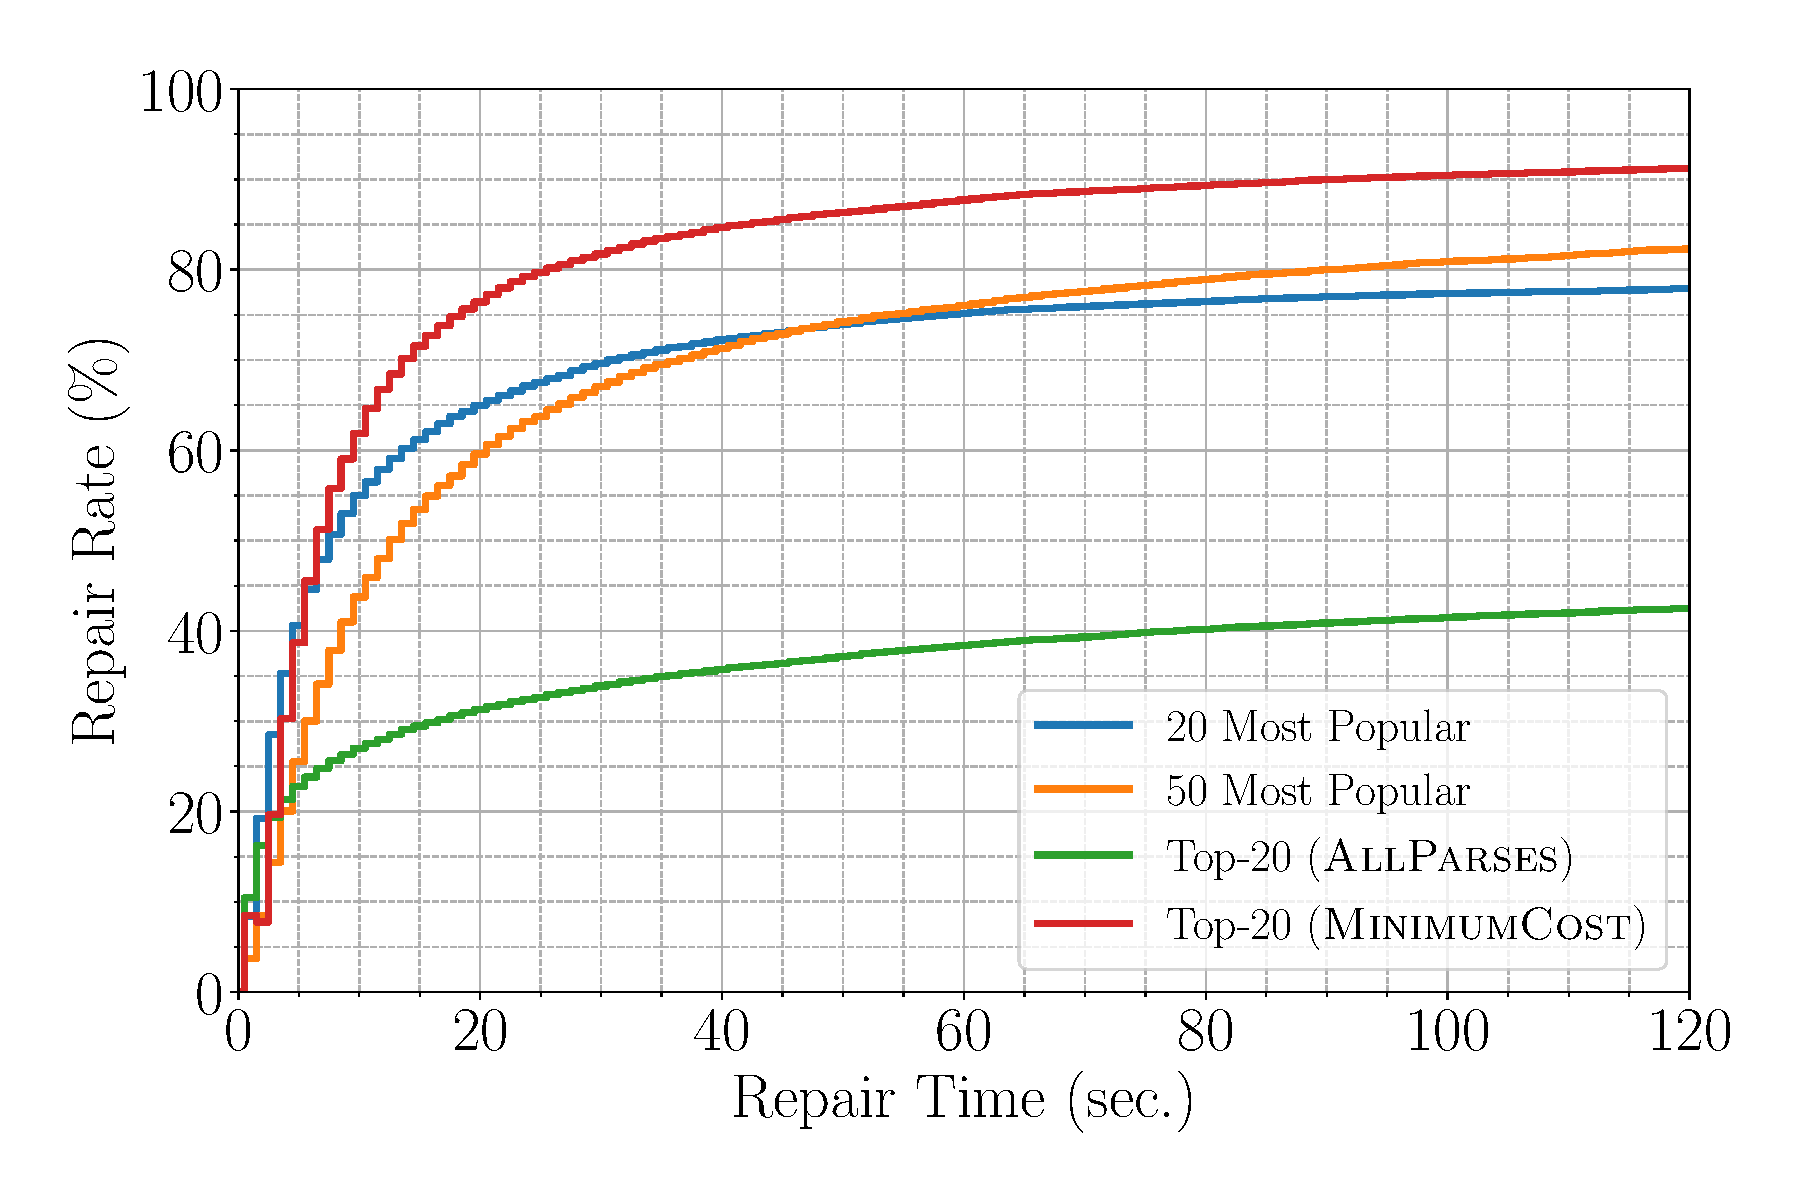
\includegraphics[width=0.7\linewidth]{tool-repair-rate.pdf}
  \caption{The repair rate for all the approached in
  \autoref{tab:seq2parse_full_results}}
  \label{fig:tool-repair-rate}
\end{figure}

Next we evaluate \toolname's efficiency by measuring how many programs it is
able to generate a (well-typed) repair for.
%
We limit the synthesizer to 90 seconds. (In general the procedure is
undecidable, and we conjecture that a longer timeout will diminish the practical
usability for novices.)
%
Recall that the repair synthesis algorithm is guided by the repair template
predictions.
%
We evaluate the efficiency of \toolname by comparing it against a baseline
\naive implementation that, given the predicted fix location, attempts to
synthesize a repair from the trivial ``hole'' template.

\autoref{fig:rite_naive} shows the cumulative distribution function of
\toolname's and \naive's repair rates over their synthesis time. We observe that
using the predicted templates for synthesis allows \toolname to generate
type-correct repairs for almost 70\% of the programs in under 20 seconds, which
is nearly 12 points higher than the \naive baseline. We also observe that
\toolname successfully repairs around 10\% more programs than \naive for times
greater than 20 seconds. While the \naive approach is still able to synthesize
well-typed repairs relatively quickly, we will see that these repairs are of
much lower quality than those generated from the predicted templates
(\S~\ref{sec:eval:template_quality}).

\begin{framed}
  \noindent \toolname can generate type-correct repairs for the vast majority of
  ill-typed programs in under 20 seconds.
\end{framed}
